\section{Background}
\label{sec:background}

\begin{figure}[t]
\centering
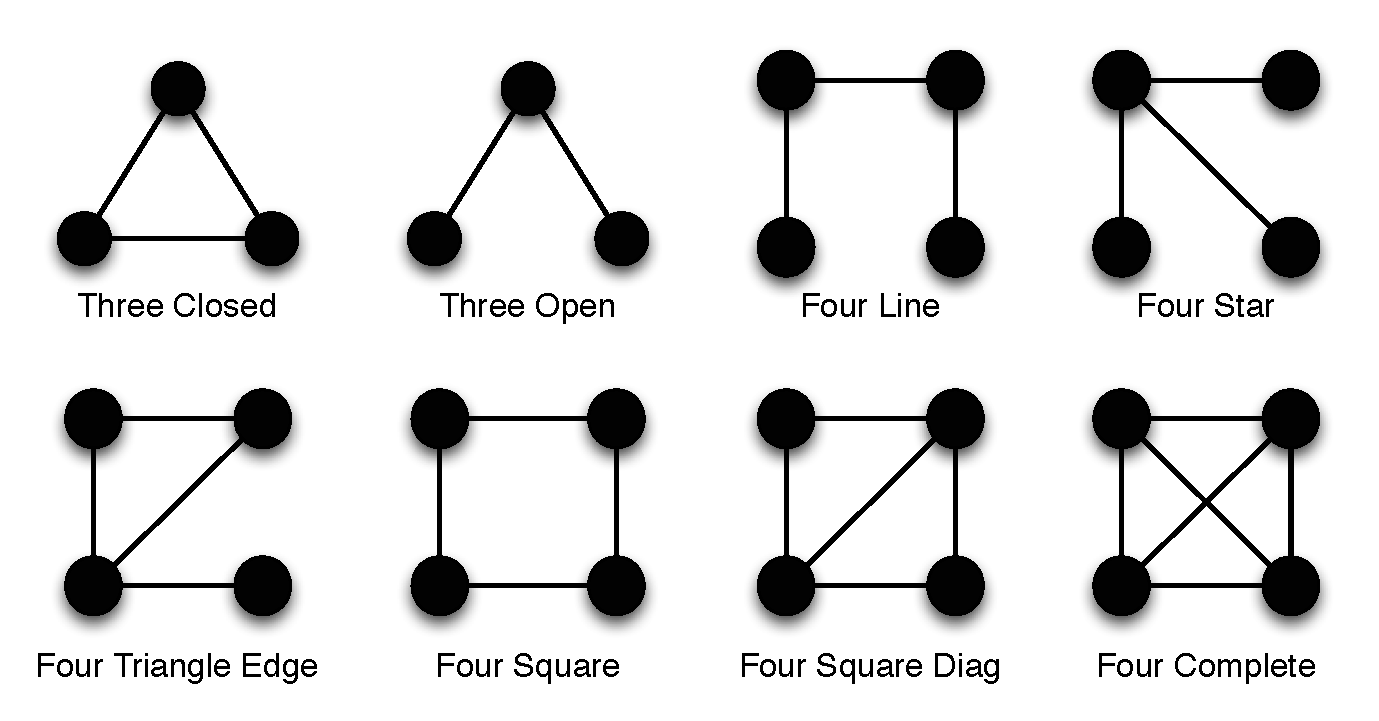
\includegraphics[width=3in]{Figures/motifs.eps}
\caption{Graphical representation of the 3-motifs and 4-motifs.}
\label{fig:motif}
\end{figure}

In this section, we first give some basic concepts that we use throughout the paper. Then, we formulate the problem of motif-driven graph generation. 

A \textbf{graph} is a representation of a set of objects and the
connections between them.  It is defined as a tuple $(V, E)$, where $V$ is
a set of $|V| = N$ vertices ("nodes") and $E \subseteq V \times V$ is a set of edges.
The nodes in a graph correspond to the objects, and the edges to
the connections.

A graph is called \textbf{simple} if no node has an edge to itself and no two
nodes have more than one edge between them.  A graph is \textbf{undirected}
if whenever $(v, w)$ is an edge, $(w, v)$ is also an edge.  In our problem, 
we assume all graphs are simple and undirected.

A \textbf{subgraph} of $G$ is a graph whose nodes and edges form subsets of 
the nodes and edges of the graph $G$.  An
\textbf{induced subgraph} of $G$ on the vertices $V' \subseteq V$ is the
graph consisting of the vertices $V'$ and the edges between them.

A \textbf{motif} is a small, connected graph, often considered as a
subgraph of a larger graph. In this paper, we only
consider motifs with $3$ or $4$ vertices, which we term "3-motifs" and
"4-motifs" respectively.  A full list of motifs is shown in
Figure~\ref{fig:motif}.

The \textbf{motif distribution} of a graph $G$ specifies how many of each
motif type the graph contains.  For example, a graph with motif
distribution \{mtThreeClosed: 12, mtThreeOpen: 16, mfFourLine: 22,
mfFourSquare: 18, mfFourStar: 30, mfFourTriangleEdge: 10, mfFourSquareDiag:
17, mfFourComplete: 2\} would contain twelve triangles, two 4-cliques, and
so forth.
